\setlength{\parskip}{0.125in}

\chapter{Объявление о проведении Конкурса}

Общество с ограниченной ответственностью <<Мэйл.Ру>>, созданное и действующее в соответствии с законодательством Российской Федерации, с
местом нахождения по адресу: 125167, г. Москва, Ленинградский проспект, д. 39, строение 79, далее по тексту <<Организатор конкурса>>,
приглашает физических лиц, достигших к моменту опубликования настоящего Объявления о конкурсе 18 лет, далее по тексту <<Участник конкурса>>,
к участию в конкурсе на нижеследующих условиях:

\section{Наименование Конкурса}

<<Российский кубок по программированию искусственного интеллекта (Russian AI Cup)>>.

Целями проведения Конкурса являются:
\begin{itemize}
\item повышение общественного интереса к сфере создания программных продуктов;
\item предоставление Участникам конкурса возможности раскрыть творческие способности;
\item развитие профессиональных навыков Участников конкурса.
\end{itemize}

Конкурс состоит из 3 (трёх) этапов, каждый из которых завершается определением Победителей. Последний этап Конкурса является решающим для
Участников конкурса в состязании за получение звания Победителя Конкурса, занявшего соответствующее призовое место.

\section{Информация об организаторе конкурса}

Наименование: ООО <<Мэйл.Ру>>

Адрес места нахождения: 125167, г. Москва, Ленинградский проспект, д. 39, строение 79

Почтовый адрес: 125167, г. Москва, Ленинградский проспект, д. 39, строение 79, БЦ <<SkyLight>>

Телефон: (495) 725-63-57

Сайт: http://www.russianaicup.ru

Е-мейл: russianaicup@corp.mail.ru

\section{Сроки проведения Конкурса}

Срок проведения Конкурса: с 00.00 часов 9 ноября 2015 года до 24.00 часов 20 декабря 2015 года по Московскому времени.

Первая неделя Конкурса (с 00.00 часов 9 ноября 2015 года до 24.00 часов 15 ноября 2015 года) является тестовой. В течение этого периода
функциональность сайта и тестирующей системы Конкурса может быть неполной, а в правила могут вноситься существенные изменения.

Сроки начала и окончания этапов Конкурса:
\begin{itemize}
\item первый этап – с 00 часов 00 минут 28 ноября 2015 года до 24 часов 00 минут 29 ноября 2015 года;
\item второй этап – с 00 часов 00 минут 5 декабря 2015 года до 24 часов 00 минут 6 декабря 2015 года;
\item третий этап (заключительный) – с 00 часов 00 минут 12 декабря 2015 года до 24 часов 00 минут 13 декабря 2015 года.
\end{itemize}

\section{Условие получения статуса Участника конкурса}

Для участия в Конкурсе необходимо пройти процедуру регистрации в Системе Организатора конкурса, размещённой на сайте Организатора конкурса в
сети Интернет по адресу: http://www.russianaicup.ru.

\section{Срок регистрации Участников конкурса в Системе Организатора}

Регистрация Участников конкурса проводится с 00.00 часов 9 ноября 2015 года до 24.00 часов 20 декабря 2015 года включительно.

\section{Территория проведения Конкурса}

Конкурс проводится на территории Российской Федерации. Проведение всех этапов Конкурса осуществляется путем удалённого доступа к Системе
Организатора конкурса через сеть Интернет.

\section{Условия проведения Конкурса (существо заданий, критерии и порядок оценки)}

Порядок проведения Конкурса, существо задания, критерии и порядок оценки указаны в конкурсной документации в разделе 2.1.

Конкурсная документация включает в себя:
\begin{itemize}
\item Объявление о проведении Конкурса;
\item Соглашение об организации и порядке проведения Конкурса;
\item Правила проведения Конкурса;
\item информационные данные, содержащиеся в Системе Организатора конкурса.
\end{itemize}

Участник конкурса может ознакомиться с конкурсной документацией на сайте Организатора конкурса в сети Интернет по адресу:
http://www.russianaicup.ru, а также при прохождении процедуры регистрации в Системе Организатора конкурса.

Организатор конкурса оставляет за собой право на изменение конкурсной документации, условий проведения Конкурса и отказ от его проведения в
соответствии с условиями конкурсной документации и нормами законодательства РФ. При этом, Организатор Конкурса обязуется уведомить
Участников конкурса обо всех произошедших изменениях путём отправки уведомления, в порядке и на условиях, предусмотренных в конкурсной
документации.

\section{Порядок определения Победителей и вручения Призов. Призовой фонд Конкурса}

Критерии оценки результатов Конкурса, количество и порядок определения Победителей содержатся в разделе 2.1 данного документа.

Призовой фонд Конкурса формируется за счет средств Организатора конкурса.

Призовой фонд:
\begin{itemize}
\item 1 место --- Apple Macbook Pro 13\textquotedbl;
\item 2-3 места --- Apple Macbook Air 13\textquotedbl;
\item 4-6 места --- Apple iPad Air 2;
\item 1-3 места в квалификации (Песочница) --- WD My Passport Ultra 500 GB;
\item 4-6 места в квалификации (Песочница) --- Kingston SSD Now V300 120GB.
\end{itemize}

Все участники Конкурса, принявшие участие во втором или третьем этапах, будут награждены футболкой. Все участники Конкурса, принявшие
участие в третьем этапе, также получат толстовку с символикой соревнования.

Все участники, занявшие призовые места, будут оповещены посредством отправки сообщения на адрес электронной почты, указанный участником при
регистрации в Системе Организатора.

Призы будут высланы участникам в виде посылок, используя Почту России или другую почтовую службу, в течение двух месяцев после окончания
финального этапа. Срок доставки приза по почтовому адресу, указанному участником, зависит от сроков доставки используемой почтовой службы.
Почтовые адреса призёров для отправки призов Организатор получает из учётных данных участника в Системе Организатора. Адрес должен быть
указан участником-призёром в течение трёх дней после получения уведомления о получении приза.

При отсутствии ответа в обозначенные сроки или отказе предоставить точные данные, необходимые для вручения призов Конкурса, Организатор
оставляет за собой право отказать такому участнику в выдаче приза Конкурса. Денежный эквивалент приза не выдаётся.
 
Победители Конкурса обязуются предоставить Организатору конкурса копии всех документов, необходимых для бухгалтерской и налоговой отчётности
Организатора конкурса. Перечень документов, которые Победитель обязан предоставить Организатору конкурса, может включать в себя:
\begin{itemize}
\item копию паспорта Победителя;
\item копию свидетельства о постановке на налоговый учет Победителя;
\item копию пенсионного удостоверения Победителя;
\item данные об открытии банковского лицевого счета Победителя;
\item иные документы, которые Организатор конкурса потребует от Участника конкурса в целях формирования отчётности о проведённом Конкурсе.
\end{itemize}

Наряду с копиями Организатор конкурса вправе запросить оригиналы вышеуказанных документов.

В соответствии с подпунктом 4 пункта 1 статьи 228 НК РФ Победитель Конкурса, ставший обладателем Приза, самостоятельно несёт все расходы по
уплате всех применимых налогов, установленных действующим законодательством Российской Федерации.

\section{Порядок и способ информирования участников Конкурса}

Информирование Участников Конкурса осуществляется путём размещения информации в сети Интернет на Сайте Организатора конкурса по адресу:
http://www.russianaicup.ru, а также через Систему Организатора конкурса, в течение всего срока проведения Конкурса.

\chapter{О мире CodeRacing 2015}

\section{Общие положения игры и правила проведения турнира}

Данное соревнование предоставляет вам возможность проверить свои навыки программирования, создав искусственный интеллект (стратегию),
управляющий одним или группой из двух кодемобилей в специальном игровом мире (подробнее об особенностях мира CodeRacing 2015 можно узнать в
следующих разделах). В каждой игре вам будет противостоять одна или несколько стратегий других игроков. Основной целью каждого кодемобиля
является максимально быстрое прохождение $2$ кругов замкнутой трассы. За каждый пройденный круг и дополнительно, после завершения
второго, кодемобиль зарабатывает баллы, необходимые вам для победы. Однако даже в гонках <<Формулы-1>> иногда применяются не совсем
честные действия, не оптимальные для одиночного прохождения трассы, но мешающие соперникам в групповом заезде добраться до финиша раньше
вас. В мире кодемобилей подобные <<грязные>> приёмы не просто являются нормой, но и разрешены официально. Вы можете мешать вашему сопернику,
наносить ему повреждения различными способами и даже временно выводить из строя его кодемобиль, получая за это дополнительные баллы. Звание
победителя игры, а также все остальные места распределяются в соответствии с количеством набранных баллов. Два или более игроков могут
делить одно место, если их баллы равны.

Турнир проводится в несколько этапов, которым предшествует квалификация в Песочнице. Песочница --- соревнование, которое проходит на
протяжении всего чемпионата. В рамках каждого этапа игроку соответствует некоторое значение рейтинга --- показателя того, насколько успешно
его стратегия участвует в играх.

Начальное значение рейтинга в Песочнице равно $1200$. По итогам игры это значение может как увеличиться, так и уменьшиться. При этом победа
над слабым (с низким рейтингом) противником даёт небольшой прирост, также и поражение от сильного соперника незначительно уменьшает ваш
рейтинг. Со временем рейтинг в Песочнице становится всё более инертным, что позволяет уменьшить влияние случайных длинных серий побед или
поражений на место участника, однако вместе с тем и затрудняет изменение его положения при существенном улучшении стратегии. Для отмены
данного эффекта участник может сбросить изменчивость рейтинга до начального состояния при отправке новой стратегии, включив соответствующую
опцию. В случае принятия новой стратегии системой рейтинг участника мгновенно упадёт, однако по мере участия в играх быстро восстановится и
даже станет выше, если ваша стратегия действительно стала эффективнее. Не рекомендуется использовать данную опцию при незначительных,
инкрементальных улучшениях вашей стратегии, а также в случаях, когда новая стратегия недостаточно протестирована и эффект от изменений в
ней достоверно не известен.

Начальное значение рейтинга на каждом основном этапе турнира равно $0$. За каждую игру участник получает определённое количество единиц
рейтинга в зависимости от занятого в бою места (система, аналогичная используемой в чемпионате <<Формула-1>>). Если двое или более
участников делят какое-то место, то суммарное количество единиц рейтинга за это место и за следующие
$\texttt{количество\_таких\_участников}-1$ мест делится поровну между этими участниками. Например, если двое участников делят третье место,
то каждый из них получит половину от суммы единиц рейтинга за третье и четвёртое места. При делении округление всегда совершается в меньшую
сторону. Более подробная информация об этапах турнира будет представлена в анонсах на сайте проекта.

Сначала все участники могут участвовать только в играх, проходящих в Песочнице. Игроки могут отправлять в Песочницу свои стратегии, и
последняя принятая из них берётся системой для участия в квалификационных играх. Каждый игрок участвует примерно в одной квалификационной
игре за час. Жюри оставляет за собой право изменить этот интервал, исходя из пропускной способности тестирующей системы, однако для всех
участников он остаётся постоянной величиной. Игры в Песочнице проходят по правилам, соответствующим правилам случайного прошедшего этапа
турнира или же правилам следующего (текущего) этапа. При этом, чем ближе значение рейтинга двух игроков в рамках Песочницы, тем больше
вероятность того, что они окажутся в одной игре. Песочница стартует до начала первого этапа турнира и завершается через некоторое время
после финального (смотрите расписание этапов для уточнения подробностей). Помимо этого Песочница замораживается на время проведения этапов
турнира. По итогам игр в Песочнице происходит отбор для участия в Раунде $1$, в который пройдут $900$ участников с наибольшим рейтингом (при
его равенстве приоритет отдаётся игроку, раньше отправившему последнюю версию своей стратегии).

Этапы турнира:
\begin{itemize}
  \item В Раунде $1$ вам предстоит освоить базовое управление кодемобилем на небольшом наборе гоночных трасс, а также изучить некоторые
        особенности кодемобиля багги. В каждой игре данного этапа примет участие $4$ игрока, у которых будет по одному кодемобилю указанного
        типа. Этот этап, как и все последующие, состоит из двух частей, между которыми будет небольшой перерыв (с возобновлением работы
        Песочницы), который позволит улучшить свою стратегию. Для игр в каждой части выбирается последняя стратегия, отправленная игроком до
        начала этой части. Игры проводятся волнами. В каждой волне каждый игрок участвует ровно в одной игре. Количество волн в каждой части
        определяется возможностями тестирующей системы, но гарантируется, что оно не будет меньше десяти. $300$ участников с наиболее
        высоким рейтингом пройдут в Раунд $2$. Также в Раунд $2$ будет проведён добор $60$ участников с наибольшим рейтингом в Песочнице (на
        момент начала Раунда $2$) из числа тех, кто не прошёл по итогам Раунда $1$.
  \item В Раунде $2$ вам предстоит улучшить свои навыки управления кодемобилем, освоить расширенный набор трасс, а также изучить некоторые
        особенности другого кодемобиля --- джипа. Так же, как и в предыдущем этапе, игры будут проходить в формате $4\times1$ --- $4$
        игрока, по одному кодемобилю у каждого. Между этапами будет некоторый перерыв, позволяющий доработать стратегию. Усложняет задачу
        то, что после подведения итогов Раунда $1$ часть слабых стратегий будет отсеяна и вам придётся противостоять более сильным
        соперникам. По итогам Раунда $2$ лучшие $50$ стратегий попадут в Финал. Также в Финал будет проведен добор $10$ участников с
        наибольшим рейтингом в Песочнице (на момент начала Финала) из числа тех, кто не прошёл в рамках основного турнира.
  \item Финал является самым серьёзным этапом. После отбора, проведённого по итогам двух первых этапов, останутся сильнейшие. И в каждой
        игре вам придётся сойтись лицом к лицу с одним из них. Для победы вам необходимо не только обобщить навыки управления различными
        кодемобилями, полученные на предыдущих этапах соревнования, но также и реализовать координацию действий ваших кодемобилей. Только
        слаженная работа приведёт вашу команду к желаемому результату. Дополнительную сложность представляет то, что трассы Финала не будут
        известны заранее, а стратегиям участников придётся принимать решения в условиях частичной видимости. Игры Финала будут проходить в
        формате $2\times2$ --- $2$ игрока, по одному кодемобилю каждого типа у каждого игрока. Система проведения Финала имеет свои
        особенности. Этап по-прежнему делится на две части, однако они уже не будут состоять из волн. Для каждой пары участников Финала
        будет проведено две игры. Гоночные трассы не являются симметричными. Поэтому в целях уменьшения влияния начальной позиции
        кодемобилей на результат игры вторая из этих игр будет отличаться от первой лишь тем, что кодемобили участников поменяются местами
        (багги первого участника поменяется местом с багги второго, соответственно и джипы обоих участников поменяются местами между собой).
        Если позволит время и возможности тестирующей системы, описанная серия игр будет повторена.
\end{itemize}

После окончания Финала все финалисты упорядочиваются по невозрастанию рейтинга. При равенстве рейтингов более высокое место занимает тот
финалист, чья участвовавшая в финале стратегия была отослана раньше. Призы за Финал распределяются на основании занятого места после этого
упорядочивания. Лучшие шесть финалистов награждаются призами:
\begin{itemize}
\item 1 место --- Apple Macbook Pro 13\textquotedbl;
\item 2-3 места --- Apple Macbook Air 13\textquotedbl;
\item 4-6 места --- Apple iPad Air 2;
\end{itemize}

После окончания Песочницы все её участники, кроме призёров Финала, упорядочиваются по невозрастанию рейтинга. При равенстве рейтингов более
высокое место занимает тот участник, который раньше отослал последнюю версию своей стратегии. Призы за Песочницу распределяются на основании
занятого места после этого упорядочивания. Лучшие шесть участников Песочницы награждаются ценными подарками.

\section{Описание игрового мира}

Игровой мир является двумерным. Ось абсцисс в этом мире направлена слева направо, ось ординат --- сверху вниз, угол $0.0$ совпадает с
направлением оси абсцисс, а положительный угол вращения означает вращение по часовой стрелке. Гоночная трасса может быть представлена в виде
прямоугольной матрицы, элементами которой являются <<тайлы>>. Каждое из измерений матрицы (количество строк и количество столбцов) находится
в интервале от $8$ до $16$ включительно. Тайл --- это квадратная область размером $800\times800$. В игре есть $12$ типов тайлов: $4$
поворота (например, \texttt{LEFT\_TOP\_CORNER}), $4$ Т-образных перекрёстка (например, \texttt{LEFT\_HEADED\_T}), прямой вертикальный
участок дороги (\texttt{VERTICAL}), прямой горизонтальный участок дороги (\texttt{HORIZONTAL}), перекрёсток (\texttt{CROSSROADS}), а также
тайл, не содержащий участка дороги (\texttt{EMPTY}). Отступ от границы тайла до прямого участка трассы, проходящего через этот тайл, равен
$80$. Радиус всех закруглений участков трассы также равен $80$. Все тайлы одного типа полностью идентичны друг другу.

Далее приведены схемы некоторых тайлов:
\begin{itemize}
\newpage
\item Схема тайла типа \texttt{LEFT\_TOP\_CORNER}, служащего для соединения двух других непустых тайлов --- справа и снизу от данного.
Другие три поворота могут быть получены путём вращения данного тайла в плоскости игрового мира с шагом $90^\circ$.
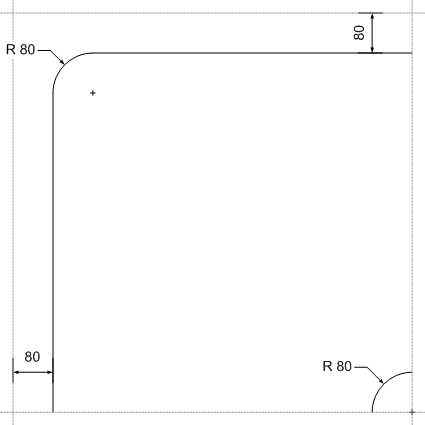
\includegraphics{images/tiles/LeftTopCorner.png}

\newpage
\item Схема тайла типа \texttt{LEFT\_HEADED\_T}, служащего для соединения трёх других непустых тайлов --- слева, сверху и снизу от данного.
Другие три Т-образных участка дороги могут быть получены путём вращения данного тайла с шагом $90^\circ$.
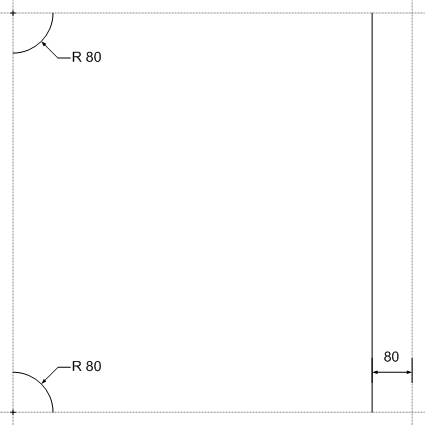
\includegraphics{images/tiles/LeftHeadedT.png}

\newpage
\item Схема вертикального участка дороги, горизонтальный участок может быть получен из него путём вращения на $90^\circ$ в любую сторону.
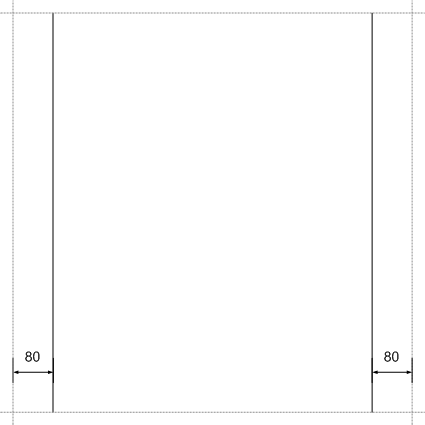
\includegraphics{images/tiles/Vertical.png}

\newpage
\item Схема перекрёстка.
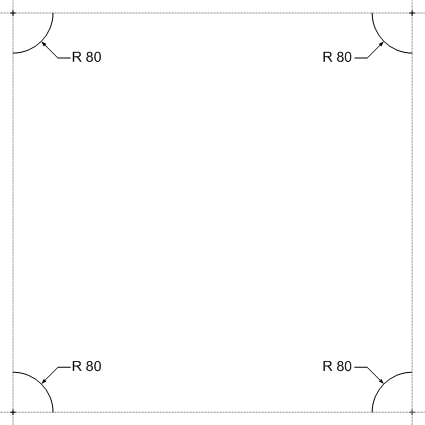
\includegraphics{images/tiles/Crossroads.png}
\end{itemize}

Время в игре дискретное и измеряется в <<тиках>>. В начале каждого тика игра получает от стратегий желаемые действия кодемобилей в этот тик
и обновляет состояние кодемобилей в соответствии с этими желаниями и ограничениями мира. Затем происходит расчёт изменения мира и объектов в
нём за этот тик, и процесс повторяется снова с обновлёнными данными. Базовая длительность каждой игры определяется эвристическим алгоритмом
и примерно пропорциональна длине и сложности гоночной трассы. Как правило, она находится в интервале от $5000$ до $15000$ тиков. К
полученному значению прибавляется $180$ --- количество тиков в начале игры, в течение которых стратегия получает управление кодемобилем,
однако не может изменять его положение и скорость. Если какой-либо кодемобиль финиширует (завершает второй круг трассы), то для остальных
кодемобилей с текущего момента устанавливается дедлайн, равный $20\%$ базовой длительности игры и округлённый вниз до целого количества
тиков. Если в течение этого времени ни один кодемобиль не придёт к финишу, игра завершается преждевременно. В противном случае после каждого
финишировавшего кодемобиля будет установлен новый дедлайн. Установка дедлайна не может продлить игру свыше её базовой длительности. Если для
каждого кодемобиля верно, что он финишировал трассу либо стратегия, управляющая им, <<упала>>, игра завершается преждевременно.

<<Упавшая>> стратегия больше не может управлять кодемобилями. Стратегия считается <<упавшей>> в следующих случаях:
\begin{itemize}
  \item Процесс, в котором запущена стратегия, непредвиденно завершился, либо произошла ошибка в протоколе взаимодействия между стратегией
        и игровым сервером.
  \item Стратегия превысила одно (любое) из отведённых ей ограничений по времени. Стратегии на один тик выделяется не более $5$ секунд
        реального времени. Но в сумме на всю игру процессу стратегии выделяется
        \begin{equation}
        30\times\textit{<длительность\_игры\_в\_тиках>}\times\textit{<количество\_кодемобилей\_в\_команде>}+5000
        \end{equation}
        миллисекунд реального времени и
        \begin{equation}
        15\times\textit{<длительность\_игры\_в\_тиках>}\times\textit{<количество\_кодемобилей\_в\_команде>}+5000
        \end{equation}
        миллисекунд процессорного времени. \footnote[1]{Несмотря на то, что ограничение реального времени заметно выше ограничения
        процессорного времени, запрещено искусственно <<замедлять>> тестирование стратегии командами типа <<\texttt{sleep}>> (равно как и
        пытаться замедлить/дестабилизировать тестирующую систему другими способами). В случае выявления подобных злоупотреблений, жюри
        оставляет за собой право применить к данному пользователю меры на своё усмотрение, вплоть до дисквалификации из соревнования и
        блокировки аккаунта.} В формуле учитывается только базовая длительность игры. Ограничение по времени остаётся прежним, даже если
        реальная длительность игры отличается от этого значения. Все ограничения по времени распространяются не только на код участника, но
        и на взаимодействие клиента-оболочки стратегии с игровым симулятором.
  \item Стратегия превысила ограничение по памяти. В любой момент времени процесс стратегии не должен потреблять более 256 Мб оперативной
        памяти.
\end{itemize}

Гонки Финала будут проходить в режиме частичной видимости. По умолчанию в каждой ячейке матрицы тайлов гоночной трассы будет находиться
специальное значение \texttt{UNKNOWN}, показывающее, что тип тайла вам (пока) не известен. Тайлы будут открываться по мере прохождения
трассы, и в большинстве случаев вся трасса станет известна вам после завершения первого круга. В каждый тик кодемобиль открывает тайл, в
котором он непосредственно находится, а также все тайлы, манхэттенское расстояние которых от данного тайла не превышает $2$ --- всего до
$13$ тайлов. Стратегия участника будет получать данные обо всех юнитах, находящихся в открытых тайлах, но не о юнитах в тайлах со значением
\texttt{UNKNOWN}.

Физика игрового мира основана на движке Notreal2D, специально разработанном для CodeRacing 2015 и других проектов серии Russian AI Cup.
Исходный код Notreal2D опубликован на Github: https://github.com/Russian-AI-Cup/notreal2d.

\section{Описание типов юнитов}

В мире CodeRacing 2015 существует $4$ типа юнитов: кодемобили, снаряды, бонусы и лужи мазута. В свою очередь существует два типа
кодемобилей: багги (\texttt{BUGGY}) и джип (\texttt{JEEP}); два типа снарядов: шайба (\texttt{WASHER}) и шина (\texttt{TIRE}); а также пять
типов бонусов: ремкомплект (\texttt{REPAIR\_KIT}), ящик со снарядами (\texttt{AMMO\_CRATE}), заряд для системы закиси азота
(\texttt{NITRO\_BOOST}), канистра с мазутом (\texttt{OIL\_CANISTER}) и дополнительные баллы (\texttt{PURE\_SCORE}). Сравнительные
массогабаритные характеристики юнитов приведены в следующей таблице:

\begin{tabular}{| l | l | l | l | l | l | l |}
  \hline
  Характеристика юнита & Багги    & Джип     & Шайба & Шина   & Бонус    & Лужа мазута \\
  \hline
  Форма                & прямоуг. & прямоуг. & круг  & круг   & прямоуг. & круг        \\
  Ширина/диаметр       & $210$    & $210$    & $40$  & $140$  & $70$     & $300$       \\
  Высота               & $140$    & $140$    & ---   & ---    & $70$     & ---         \\
  Масса                & $1250$   & $1500$   & $10$  & $1000$ & $100$    & ---         \\
  \hline
\end{tabular}

\section{Характеристики и управление кодемобилем}

Основной характеристикой кодемобиля является прочность. Начальная (и максимальная) прочность каждого кодемобиля равна $1.0$. Если прочность
падает до нуля, кодемобиль считается выведенным из строя и перестаёт управляться стратегией. Однако через $300$ тиков кодемобиль
восстанавливается (его прочность становится равной $1.0$) и может продолжать движение.

Скорость и направление движения кодемобиля определяются следующими тремя параметрами:
\begin{itemize}
  \item Относительная мощность работы двигателя \texttt{car.enginePower}. Значение находится в интервале от $-1.0$ до $1.0$ кроме случаев,
        когда кодемобиль использует ускорение <<нитро>>. При переходе кодемобиля в режим ускорения относительная мощность его двигателя
        мгновенно становится равной $2.0$ и не меняется до окончания действия ускорения, затем она устанавливается в $1.0$. Абсолютная
        мощность двигателя равномерно изменяется на интервале (относительной мощности) от $-\infty$ до $0.0$ и на интервале от $0.0$ до
        $+\infty$ и для каждого типа кодемобилей подобрана таким образом, что при значении \texttt{car.enginePower}, равном $1.0$, ускорение
        кодемобиля составляет $0.25$ тиков$^{-2}$ (ускорение вперёд/замедление движения назад), а при значении $-1.0$ --- $-0.1875$
        тиков$^{-2}$ (замедление движения вперёд/ускорение назад). В игре нет явного ограничения на скорость движения кодемобилей, однако
        присутствует сопротивление воздуха, которое ограничивает их скорость естественным образом. Стратегия может установить
        \texttt{move.enginePower} --- желаемое значение относительной мощности работы, однако изменение \texttt{car.enginePower} не будет
        превышать по модулю $0.025$ за тик (кроме входа и выхода из режима ускорения).
  \item Относительный поворот руля/колёс \texttt{car.wheelTurn}. Значение находится в интервале от $-1.0$ до $1.0$ и, как и
        \texttt{car.enginePower}, не может изменяться мгновенно, а двигается к желаемому значению \texttt{move.wheelTurn} со скоростью, не
        превышающей по модулю $0.05$ за тик. Ненулевой поворот колёс порождает составляющую угловой скорости кодемобиля, значение которой
        прямо пропорционально \texttt{car.wheelTurn}, коэффициенту \texttt{game.carAngularSpeedFactor}, а также скалярному произведению
        вектора скорости кодемобиля и единичного вектора, направление которого совпадает с направлением кодемобиля. Однако реальная угловая
        скорость может отличаться от данного значения вследствие столкновений кодемобиля с другими игровыми объектами.
  \item Положение педали тормоза. В любой тик стратегия может установить флажок \texttt{move.brake}. Это действие заблокирует колёса
        кодемобиля в данный тик и увеличит силу трения, воздействующую на кодемобиль вдоль его продольной оси, до значения силы трения,
        воздействующей на кодемобиль вдоль его поперечной оси. По умолчанию первая значительно меньше второй. Блокировка колёс означает, что
        игра будет игнорировать мощность работы двигателя кодемобиля, однако стратегия по прежнему сможет изменять это значение. Данное
        состояние кодемобиля схоже с состоянием в первые $180$ тиков игры с тем исключением, что при нажатии педали тормоза у кодемобиля уже
        может быть ненулевая скорость.
\end{itemize}

У кодемобиля в распоряжении есть $3$ типа расходников: метательные снаряды (их количество равно \texttt{car.projectileCount}), заряды для
системы закиси азота (\texttt{car.nitroChargeCount}) и канистры с мазутом (\texttt{car.oilCanisterCount}). В начале игры у кодемобиля есть
по одному расходнику каждого типа. При завершении очередного круга трассы количество расходников каждого типа у кодемобиля увеличивается на
единицу. При подборе кодемобилем бонуса, содержащего расходники, количество расходников соответствующего типа увеличивается на единицу.

\begin{itemize}
  \item Стратегия может использовать метательные снаряды для нанесения повреждений и препятствования перемещению других кодемобилей. В
        момент появления центр снаряда совпадает с центром кодемобиля, запустившего этот снаряд. Разумеется, кодемобиль при этом является
        <<прозрачным>> для снаряда. Игра игнорирует пересечения и столкновения кодемобиля и запущенного им снаряда до тех пор, пока снаряд
        не столкнётся с любым другим объектом. После этого снаряд начинает взаимодействовать со всеми кодемобилями одинаково.
        \begin{itemize}
          \item В распоряжении багги находятся небольшие и лёгкие шайбы. Багги одновременно запускает три таких шайбы (тратится один
                расходник): направление первой совпадает с направлением кодемобиля, а направление двух других отличается на $+2^\circ$ и
                $-2^\circ$. Модуль скорости каждой шайбы постоянен и равен $60$ тикам$^{-1}$. Шайбы не взаимодействуют между собой и с
                какими-либо объектами, кроме кодемобилей и шин, а также проходят сквозь границы трассы. При попадании в кодемобиль шайба
                понижает его прочность на $0.15$. При столкновении с шиной шайба убирается из игрового мира.
          \item Джип использует в качестве снарядов огромные шины. Начальная скорость этого типа снарядов также равна $60$ тикам$^{-1}$.
                Шины могут отскакивать друг от друга, от кодемобилей и бортов трассы, теряя при этом часть скорости. Если скорость шины
                падает до $25\%$ от начальной, шина убирается из игрового мира. При столкновении с кодемобилем шина наносит ему урон, равный
                $35\%$ от отношения скорости соударения\footnote[2]{Здесь и далее под скоростью соударения юнитов А и Б понимается величина
                скалярного произведения вектора, полученного в результате вычитания вектора скорости юнита А в точке столкновения из вектора
                скорости юнита Б в точке столкновения, и нормали столкновения этих двух юнитов. Скорость юнита в произвольной точке
                определяется его поступательной скоростью, а также скоростью его вращения и расстоянием от центра юнита до указанной точки.
                Нормаль столкновения является единичным вектором, направление которого совпадает либо с нормалью к поверхности юнита Б в
                точке столкновения, направленной за пределы этого объекта, либо с нормалью к поверхности юнита А в точке соударения,
                направленной внутрь этого объекта. Определение нормали столкновения в каждом конкретном случае зависит от особенностей
                реализации физики игрового мира, однако для выпуклых объектов с некоторым упрощением можно считать, что направление этого
                вектора не сильно отличается от направления вектора, направленного из центра юнита Б в центр юнита А.} к начальной скорости
                снаряда.
        \end{itemize}
        После запуска очередного снаряда следующий может быть запущен не ранее, чем через $60$ тиков.
  \item При использовании ускорения <<нитро>> мощность двигателя кодемобиля мгновенно становится равной $2.0$ и не может быть изменена в
        течение $120$ тиков --- длительности ускорения. Разумеется, в течение этого времени кодемобиль не может совершить ещё одну активацию
        режима ускорения.
  \item Канистры с мазутом используются для создания дополнительных препятствий оппонентам, следующим за вашим кодемобилем на небольшой
        дистанции. При использовании расходника данного типа позади кодемобиля образуется скользкая лужа мазута. Центр лужи находится на
        продольной оси кодемобиля, а расстояние между ближайшими точками кодемобиля и лужи равно $10.0$. Лужа мазута полностью высыхает и
        убирается из игрового мира через $600$ тиков. Если какой-либо кодемобиль попадает в лужу мазута (расстояние от центра кодемобиля до
        центра лужи становится меньше её радиуса), то вследствие ухудшения сцепления колёс и поверхности дороги кодемобиль начинает
        <<заносить>>, к его угловой скорости мгновенно прибавляется некоторое случайное значение, пропорциональное модулю текущей линейной
        скорости кодемобиля, а часть мазута попадает на колёса и остаётся там некоторое время: до $60$ тиков, но не более оставшегося
        времени высыхания лужи. При этом, время высыхания лужи сокращается на то же значение. Пока на колёсах остаётся мазут, сила трения
        поверхности, воздействующая на кодемобиль, значительно уменьшается, а педаль тормоза перестаёт эффективно работать; новое попадание
        в лужу мазута до окончания этого срока не имеет никакого эффекта. Канистры с мазутом могут использоваться не чаще, чем раз в $120$
        тиков.
\end{itemize}

\section{Столкновения юнитов}

Юниты могут сталкиваться с границами трассы, а также между собой в зависимости от типов этих юнитов. При столкновении объектов модуль и
направление их скоростей меняются определённым образом в зависимости от масс и исходных скоростей объектов. Столкновения не являются
абсолютно упругими, и объекты теряют часть скорости.

Во время гонки кодемобили сталкиваются с границами трассы и всеми юнитами, кроме луж мазута. Финишировавшие кодемобили не убираются из
игрового мира, однако перестают взаимодействовать с какими-либо объектами, кроме границ трассы.

\begin{itemize}
  \item При столкновении двух кодемобилей оба кодемобиля могут получить некоторый урон. Урон, полученный кодемобилем, пропорционален
        скорости соударения и отношению массы другого кодемобиля к массе данного кодемобиля. Если урон меньше, чем $0.01$, то он
        игнорируется.
  \item При столкновении с ограждением трассы кодемобиль получает урон, пропорциональный скорости соударения. Как и в случае со
        столкновением двух кодемобилей, урон ниже $0.01$ считается несущественным и игнорируется.
  \item При столкновении со снарядом кодемобиль получает урон в зависимости от типа снаряда. Подробная информация о столкновениях этого типа
        уже приводилась ранее.
  \item После столкновения кодемобиля с бонусом последний убирается из игрового мира, а кодемобиль или его владелец получают некоторое
        вознаграждение, в зависимости от типа бонуса:
        \begin{itemize}
          \item Ремкомплект полностью восстанавливает прочность кодемобиля.
          \item Ящик со снарядами, заряд для системы закиси азота и канистра с мазутом увеличивают количество расходников соответствующего
                типа в распоряжении кодемобиля на единицу.
          \item Дополнительные баллы добавляют $100$ к счётчику баллов игрока.
        \end{itemize}
  \item Лужи мазута не взаимодействуют с кодемобилями и любыми другими юнитами как физические объекты. Подробная информация о воздействии
        лужи мазута на кодемобиль уже приводилась ранее.
\end{itemize}

Все типы столкновений, не описанные в данном документе, игнорируются симулятором игры.

\section{Прохождение трассы и начисление баллов}

Прохождение одного круга трассы заключается в последовательном посещении всех ключевых тайлов (\texttt{world.waypoints}) и возврате в
начальный тайл. Тайл считается посещённым, как только центр кодемобиля пересекает границу тайла. Вероятность точного совпадения центра
кодемобиля и границы тайла крайне мала, но для полного соблюдения всех формальностей стоит отметить, что тайл включает в себя левую и
верхнюю границы, правая и нижняя принадлежат соседним тайлам. За полное прохождение круга кодемобиль приносит игроку ровно $1000$ баллов.
При этом начисление производится не единовременно, а по мере посещения ключевых тайлов. $500$ баллов из указанной тысячи распределяются
равномерно по всем ключевым тайлам, кроме последнего. При этом используется целочисленное деление, таким образом суммарный балл за эти тайлы
может быть чуть менее $500$. Кодемобиль, первым завершивший $2$ круга, получает дополнительную премию размером в $512$ баллов. Премия за
каждое последующее финиширование трассы уменьшается вдвое.

Как уже указывалось, быстрое прохождение трассы является основным источником получения баллов. Есть и другие способы:
\begin{itemize}
  \item Подбор бонусов, содержащих баллы. $100$ баллов за каждый бонус.
  \item Нанесение повреждений кодемобилям других игроков. Повреждения учитываются с коэффициентом $100.0$. Округление производится вниз до
        ближайшего целого числа.
  \item Выведение из строя кодемобилей других игроков. За факт выведения из строя начисляются дополнительные $100$ баллов.
\end{itemize}

Количество баллов игрока равно сумме баллов, заработанных всеми его кодемобилями.

\chapter{Создание стратегии}

\section{Техническая часть}

Сперва для создания стратегии вам необходимо выбрать один из ряда поддерживаемых языков программирования\footnote[3]{Для всех языков
программирования используются 32-битные версии компиляторов/интерпретаторов.}: Java (Oracle JDK 8), C\# (Visual C\# compiler 4.0.30319+ for
.NET framework 4.5+), C++ (GNU MinGW C++ 5.1), Python 2 (Python 2.7+), Python 3 (Python 3.5+), Pascal (Free Pascal 2.6+), Ruby (JRuby
9.0.3.0+, Oracle JDK 8). Возможно, этот набор будет расширен. На сайте проекта вы можете скачать пользовательский пакет для каждого из
языков. Модифицировать в пакете разрешено лишь один файл, который и предназначен для содержания вашей стратегии, например, MyStrategy.java
(для Java) или MyStrategy.py (для Python)\footnote[4]{Исключение составляет C++, для которого можно модифицировать два файла: MyStrategy.cpp
и MyStrategy.h. Причём наличие в архиве файла MyStrategy.cpp является обязательным (иначе стратегия не скомпилируется), а наличие файла
MyStrategy.h --- опциональным. В случае его отсутствия будет использован стандартный файл из пакета.}. Все остальные файлы пакета при сборке
стратегии будут замещены стандартными версиями. Однако вы можете добавлять в стратегию свои файлы с кодом. Эти файлы должны находиться в том
же каталоге, что и основной файл стратегии. При отправке решения все они должны быть помещены в один ZIP-архив (файлы должны находиться в
корне архива). Если вы не добавляете новых файлов в пакет, достаточно отправить сам файл стратегии (с помощью диалога выбора файла) или же
вставить его код в текстовое поле.

После того, как вы отправили свою стратегию, она попадает в очередь тестирования. Система сперва попытается скомпилировать пакет с вашими
файлами, а затем, если операция прошла успешно, создаст несколько коротких (по $200$ тиков) игр разных форматов: $4\times1$ с использованием
кодемобилей багги, $4\times1$ с использованием джипов и $2\times2$. Для управления кодемобилями каждого из участников этих игр будет запущен
отдельный клиентский процесс с вашей стратегией, и для того, чтобы стратегия считалась принятой (корректной), ни один из экземпляров
стратегии не должен <<упасть>>. Игрокам в этих тестовых играх будут даны имена в формате <<\texttt{<имя\_игрока>}>>,
<<\texttt{<имя\_игрока> (2)}>>, <<\texttt{<имя\_игрока> (3)}>> и т.д.

После успешного прохождения описанного процесса ваша посылка получает статус <<Принята>>. Первая успешная посылка одновременно означает и
вашу регистрацию в Песочнице. Вам начисляется стартовый рейтинг ($1200$), и ваша стратегия начинает участвовать в периодических
квалификационных боях (смотрите описание Песочницы для получения более подробной информации). Также вам становится доступна функция создания
собственных игр, в которых в качестве соперника можно выбирать любую стратегию любого игрока (в том числе и вашу собственную), созданную до
момента вашей последнего успешной посылки. Созданные вами игры не влияют на рейтинг.

В системе присутствуют ограничения на количество посылок и пользовательских игр, а именно:
\vspace{-0.15in}
\begin{itemize}
  \item Нельзя отправлять стратегию чаще, чем три раза за пять минут.
\vspace{-0.10in}
  \item За пять минут нельзя создать более двух пользовательских игр.
\vspace{-0.10in}
\end{itemize}

Для упрощения отладки небольших изменений стратегии в системе присутствует возможность сделать тестовую посылку (флажок <<Тестовая посылка>>
на форме отправки стратегии). Тестовая посылка не отображается другим пользователям, не участвует в квалификационных играх в Песочнице и
играх в этапах турнира, также невозможно собственноручно создавать бои с её участием. Однако после принятия данной посылки система
автоматически добавляет тестовую игру с четырьмя участниками (формат $4\times1$ с использованием кодемобилей багги): непосредственно
тестовой посылкой, стратегией из раздела <<Быстрый старт>> и двумя стратегиями, которые ничего не делают. Тестовая игра видна только
участнику, сделавшему данную тестовую посылку. Базовая длительность такой тестовой игры составляет $2000$ тиков. На частоту тестовых посылок
действует то же ограничение, что и на частоту обычных посылок. Тестовые игры на частоту создания игр пользователем не влияют.

% TODO
У игроков есть возможность в специальном визуализаторе просматривать прошедшие игры. Для этого нужно нажать кнопку <<Смотреть>> в списке игр
либо нажать кнопку <<Посмотреть игру>> на странице игры.
% У игроков есть возможность в специальном визуализаторе просматривать прошедшие игры и даже игры, которые начали
% тестироваться системой, но результат их ещё не известен (в этом случае данные о ходе игры будут поступать
% в рендерер по мере обработки их системой). Для этого нужно нажать кнопку <<Смотреть>> в списке игр либо
% нажать кнопку <<Посмотреть игру>> на странице игры.

Если вы смотрите игру с участием вашей стратегии и заметили некоторую странность в её поведении, или ваша стратегия делает не то, что вы от
неё ожидали, то вы можете воспользоваться специальной утилитой Repeater для воспроизведения локального повтора данной игры. Локальный повтор
игры --- это возможность запустить стратегию на вашем компьютере так, чтобы она видела игровой мир вокруг себя таким, каким он был при
тестировании на сервере. Это поможет вам выполнять отладку, добавлять логирование и наблюдать за реакцией вашей стратегии в каждый момент
игры. Для этого скачайте Repeater с сайта CodeRacing 2015 (раздел <<Документация>> $\rightarrow$ <<Утилита Repeater>>) и разархивируйте. Для
запуска Repeater вам необходимо установленное ПО Java $7+$ Runtime Environment. Обратите внимание, что любое взаимодействие вашей стратегии
с игровым миром при локальном повторе полностью игнорируется. Это означает, что в каждый момент времени окружающий мир для стратегии в
точности совпадает с миром, каким он был в игре при тестировании на сервере и не зависит от того, какие действия ваша стратегия
предпринимает. Подробнее об утилите Repeater читайте в соответствующем разделе на сайте.

Помимо всего выше перечисленного у игроков есть возможность запускать простые тестовые игры локально на своём компьютере. Для этого
необходимо загрузить архив с утилитой Local runner из раздела сайта <<Документация>> $\rightarrow$ <<Local runner>>. Использование данной
утилиты позволит вам тестировать свою стратегию в условиях, аналогичных условиям тестовой игры на сайте, но без каких либо ограничений по
количеству создаваемых игр. Рендерер для локальных игр заметно отличается от рендерера на сайте. Все игровые объекты в нём отображаются
схематично (без использования красочных моделей). Создать локальную тестовую игру очень просто: запустите Local runner с помощью
соответствующего скрипта запуска (для Windows или *n*x систем), затем запустите свою стратегию из среды разработки (или любым другим удобным
вам способом) и смотрите игру. Во время локальных игр вы можете выполнять отладку своей стратегии, ставить точки останова. Однако следует
помнить, что Local runner ожидает отклика от стратегии не более $20$ минут. По прошествии этого времени он посчитает стратегию <<упавшей>> и
продолжит работу без неё.

\section{Управление кодемобилем}

Для каждого кодемобиля в вашей команде в начале игры создаётся отдельный экземпляр класса \texttt{MyStrategy}, в полях которого стратегия
может хранить информацию о данном кодемобиле. Общую для всей команды информацию, в зависимости от языка программирования, можно хранить в
статических полях или глобальных переменных.

Управление кодемобилем осуществляется с помощью метода \texttt{move} стратегии, который вызывается один раз за тик для каждого кодемобиля.
Методу передаются следующие параметры:
\begin{itemize}
  \item кодемобиль \texttt{self}, для которого вызывается метод;
  \item текущее состояние мира \texttt{world};
  \item набор игровых констант \texttt{game};
  \item объект \texttt{move}, устанавливая свойства которого, стратегия и определяет поведение кодемобиля.
\end{itemize}

Реализация клиента-оболочки стратегии на разных языках может отличаться, однако в общем случае не гарантируется, что при разных вызовах
метода \texttt{move} в качестве параметров ему будут переданы ссылки на одни и те же объекты. Таким образом, нельзя, например, сохранить
ссылки на объекты \texttt{world} или \texttt{player} и получать в следующие тики обновлённую информацию об этих объектах, считывая их поля.

\newpage
\section{Примеры реализации}

Далее для всех языков программирования приведены простейшие примеры стратегий, которые придают кодемобилю ускорение вперёд, а также
используют некоторые расходники. Полную документацию классов и методов для языка Java можно найти в следующих главах.

\subsection{Пример для Java}

\begin{verbatim}
import model.*;

public final class MyStrategy implements Strategy {
    @Override
    public void move(Car self, World world, Game game, Move move) {
        move.setEnginePower(1.0D);
        move.setThrowProjectile(true);
        move.setSpillOil(true);

        if (world.getTick() > game.getInitialFreezeDurationTicks()) {
            move.setUseNitro(true);
        }
    }
}
\end{verbatim}

\subsection{Пример для C\#}

\begin{verbatim}
using System;
using Com.CodeGame.CodeRacing2015.DevKit.CSharpCgdk.Model;

namespace Com.CodeGame.CodeRacing2015.DevKit.CSharpCgdk {
    public sealed class MyStrategy : IStrategy {
        public void Move(Car self, World world, Game game, Move move) {
            move.EnginePower = 1.0D;
            move.IsThrowProjectile = true;
            move.IsSpillOil = true;

            if (world.Tick > game.InitialFreezeDurationTicks) {
                move.IsUseNitro = true;
            }
        }
    }
}
\end{verbatim}

\newpage
\subsection{Пример для C++}

\begin{verbatim}
#include "MyStrategy.h"

#define PI 3.14159265358979323846
#define _USE_MATH_DEFINES

#include <cmath>
#include <cstdlib>

using namespace model;
using namespace std;

void MyStrategy::move(const Car& self, const World& world, const Game& game, Move& move) {
    move.setEnginePower(1.0);
    move.setThrowProjectile(true);
    move.setSpillOil(true);

    if (world.getTick() > game.getInitialFreezeDurationTicks()) {
        move.setUseNitro(true);
    }
}

MyStrategy::MyStrategy() { }
\end{verbatim}

\newpage
\subsection{Пример для Python 2}

В языке Python 2 имя переменной текущего кодемобиля изменено с <<\texttt{self}>> на <<\texttt{me}>>.

\begin{verbatim}
from model.Car import Car
from model.Game import Game
from model.Move import Move
from model.World import World


class MyStrategy:
    def move(self, me, world, game, move):
        """
        @type me: Car
        @type world: World
        @type game: Game
        @type move: Move
        """
        move.engine_power = 1.0
        move.throw_projectile = True
        move.spill_oil = True

        if world.tick > game.initial_freeze_duration_ticks:
            move.use_nitro = True
\end{verbatim}

\subsection{Пример для Python 3}

В языке Python 3 имя переменной текущего кодемобиля изменено с <<\texttt{self}>> на <<\texttt{me}>>.

\begin{verbatim}
from model.Car import Car
from model.Game import Game
from model.Move import Move
from model.World import World


class MyStrategy:
    def move(self, me: Car, world: World, game: Game, move: Move):
        move.engine_power = 1.0
        move.throw_projectile = True
        move.spill_oil = True

        if world.tick > game.initial_freeze_duration_ticks:
            move.use_nitro = True
\end{verbatim}

\newpage
\subsection{Пример для Pascal}

В языке Pascal имя переменной текущего кодемобиля изменено с <<\texttt{self}>> на <<\texttt{me}>>.

\begin{verbatim}
unit MyStrategy;

interface

uses
    StrategyControl, BonusControl, BonusTypeControl, CarControl, CarTypeControl, DirectionControl,
    GameControl, MoveControl, OilSlickControl, PlayerControl, ProjectileControl,
    ProjectileTypeControl, TileTypeControl, TypeControl, WorldControl;

type
    TMyStrategy = class (TStrategy)
    public
        procedure Move(me: TCar; world: TWorld; game: TGame; move: TMove); override;

    end;

implementation

uses
    Math;
    
procedure TMyStrategy.Move(me: TCar; world: TWorld; game: TGame; move: TMove);
begin
    move.SetEnginePower(1.0);
    move.SetThrowProjectile(true);
    move.SetSpillOil(true);

    if (world.GetTick() > game.GetInitialFreezeDurationTicks()) then begin
        move.SetUseNitro(true);
    end;
end;

end.
\end{verbatim}

\newpage
\subsection{Пример для Ruby}

В языке Ruby имя переменной текущего кодемобиля изменено с <<\texttt{self}>> на <<\texttt{me}>>.

\begin{verbatim}
require './model/car'
require './model/game'
require './model/move'
require './model/world'

class MyStrategy
  # @param [Car] me
  # @param [World] world
  # @param [Game] game
  # @param [Move] move
  def move(me, world, game, move)
    move.engine_power = 1.0
    move.throw_projectile = true
    move.spill_oil = true

    if world.tick > game.initial_freeze_duration_ticks
        move.use_nitro = true
    end
  end
end
\end{verbatim}
